\documentclass{standalone}
\usepackage{tikz}
\usepackage{ctex,siunitx}
\setCJKmainfont{Noto Serif CJK SC}
\usepackage{tkz-euclide}
\usepackage{amsmath}
\usetikzlibrary{patterns, calc,3d}
\usetikzlibrary {decorations.pathmorphing,decorations.pathreplacing,decorations.shapes}
\tikzset{label style/.append style={font=\small}}
\begin{document}
\small
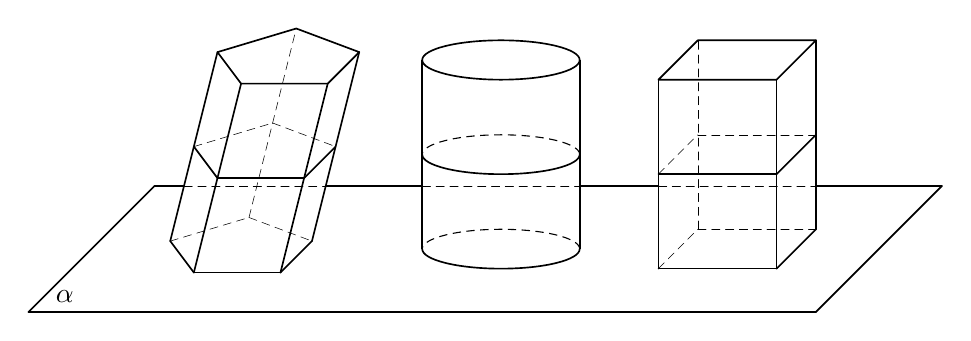
\begin{tikzpicture}[>=latex,scale=1.0]
  \tkzDefPoints{0/0/A,10/0/B,11.6/1.6/C,1.6/1.6/D,5/1.6/Ll,7/1.6/Lr,8/1.6/LL,10/1.6/LR}
  \tkzDefPoints{8/0.55/A2,9.5/0.55/B2,10/1.05/C2,8.5/1.05/D2,8/1.75/A2',8/2.95/A2''}
  \tkzDefPointsBy[translation=from A2 to A2'](B2,C2,D2){B2',C2',D2'}
  \tkzDefPointsBy[translation=from A2 to A2''](B2,C2,D2){B2'',C2'',D2''}
  \tkzDefPoints{1.8/0.9/A1,2.1/0.5/B1,3.2/0.5/C1,3.6/0.9/D1,2.8/1.2/E1,2.1/2.1/A1',2.4/3.3/A1''}
  \tkzDefPointsBy[translation=from A1 to A1'](B1,C1,D1,E1){B1',C1',D1',E1'}
  \tkzDefPointsBy[translation=from A1 to A1''](B1,C1,D1,E1){B1'',C1'',D1'',E1''}
  \tkzInterLL(C,D)(A1,A1')\tkzGetPoint{ll}
  \tkzInterLL(C,D)(D1,D1')\tkzGetPoint{lr}
  \draw[semithick](7,0.8)arc(0:-180:1 and 0.25);
  \draw[densely dashed](7,0.8)arc(0:180:1 and 0.25);
  \draw[semithick](7,2)arc(0:-180:1 and 0.25);
  \draw[densely dashed](7,2)arc(0:180:1 and 0.25);
  \draw[semithick](6,3.2)ellipse(1 and 0.25);
  \draw[semithick](7,0.8)--(7,3.2)(5,0.8)--(5,3.2);
  \tkzDrawSegments[semithick](D,A A,B B,C C,LR LL,Lr Ll,lr ll,D)
  \tkzDrawSegments[semithick](A2,B2 B2,C2 A2',B2' B2',C2' A2,A2'' B2,B2'' C2,C2'')
  \tkzDrawSegments[semithick](A1,B1 B1,C1 C1,D1 A1',B1' B1',C1' D1',C1' A1,A1'' B1,B1'' C1,C1'' D1,D1'')
  \tkzDrawPolygon[semithick](A2'',B2'',C2'',D2'')
  \tkzDrawPolygon[semithick](A1'',B1'',C1'',D1'',E1'')
  \tkzDrawSegments[densely dashed](Ll,Lr LL,LR ll,lr)
  \tkzDrawSegments[densely dashed](D2,D2'' A2,D2 D2,C2  A2',D2' D2',C2')
  \tkzDrawSegments[densely dashed](E1,E1'' A1,E1 E1,D1  A1',E1' E1',D1')
  \tkzLabelAngle[pos=0.5](B,A,D){$\alpha$};
\end{tikzpicture}
\end{document}